Grundlegend hat die Webanwendung einen hellen Style. Wir haben uns im Vorhinein für folgende Farbpalette entschieden:

\begin{figure}[h!]
    \centering
    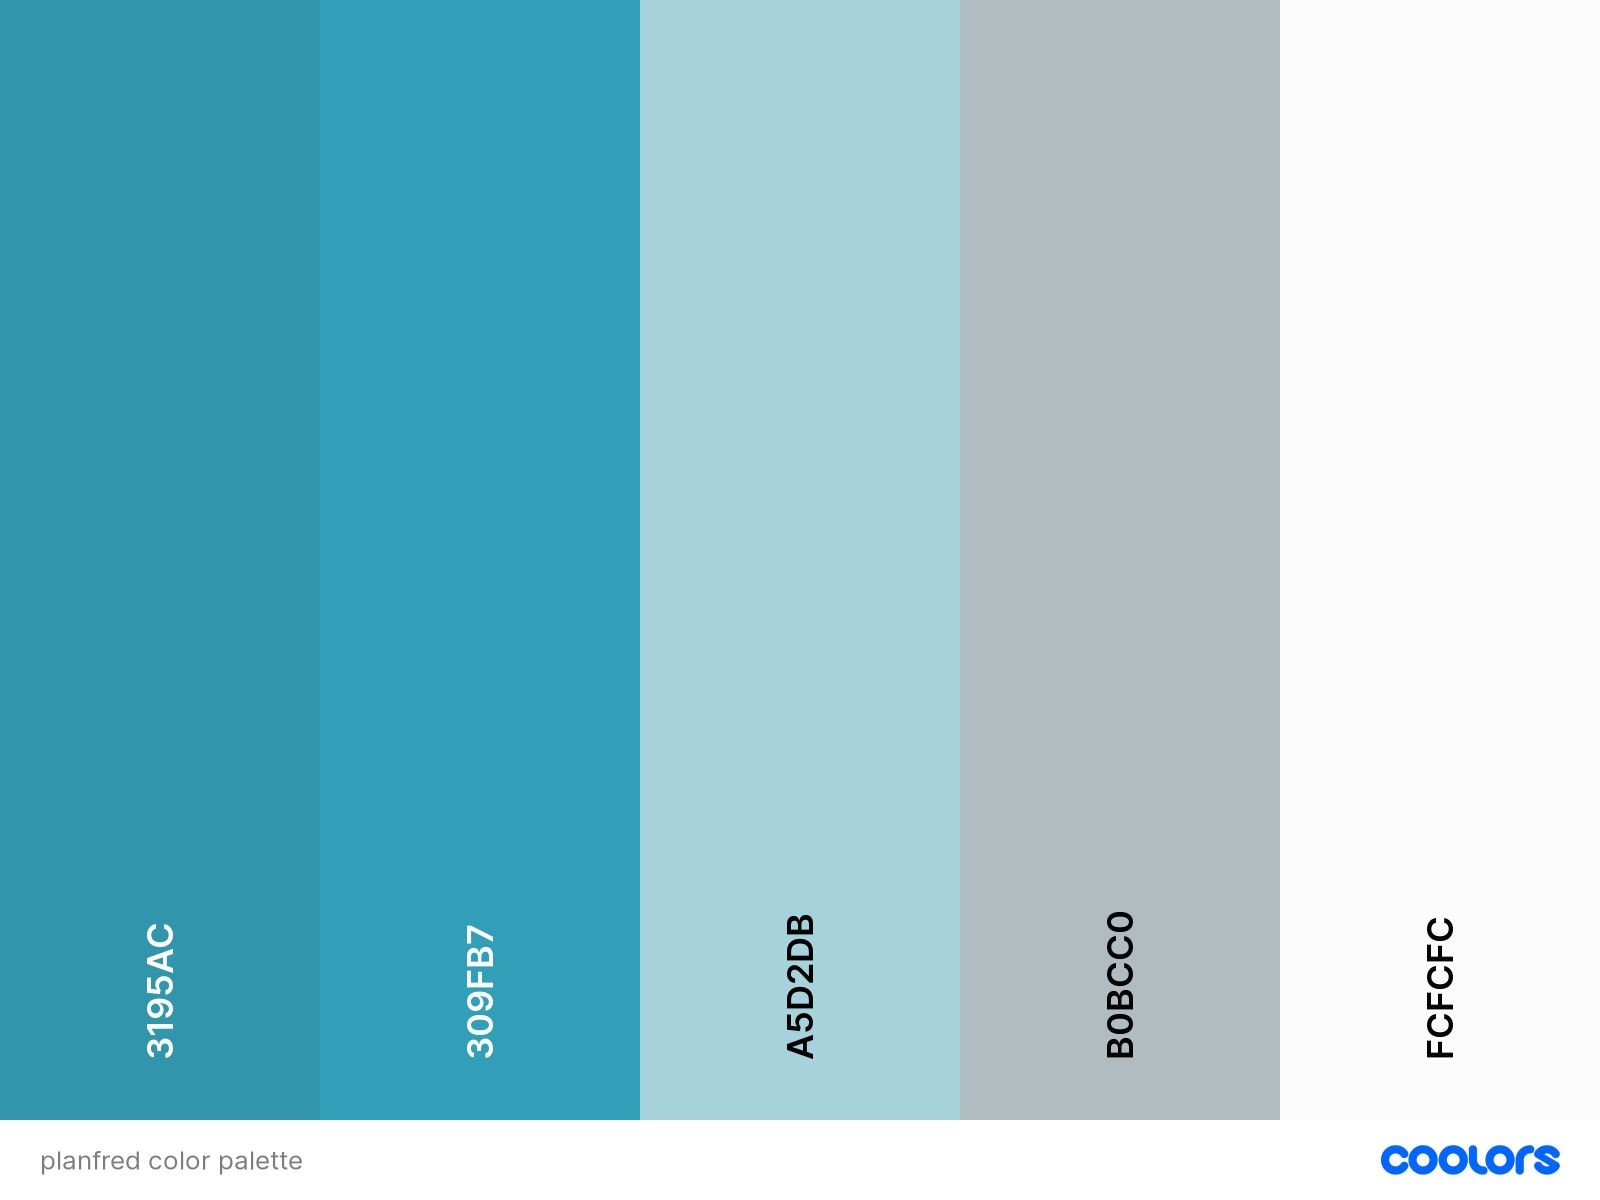
\includegraphics[width=1\textwidth]{pics/planfred-color-palette.png}
    \caption{Kundenmanagement Tool Farbpalette}
    \cite{frontend_design_colors}
    \label{fig:mesh1}
\end{figure}

\begin{figure}[h!]
    \centering
    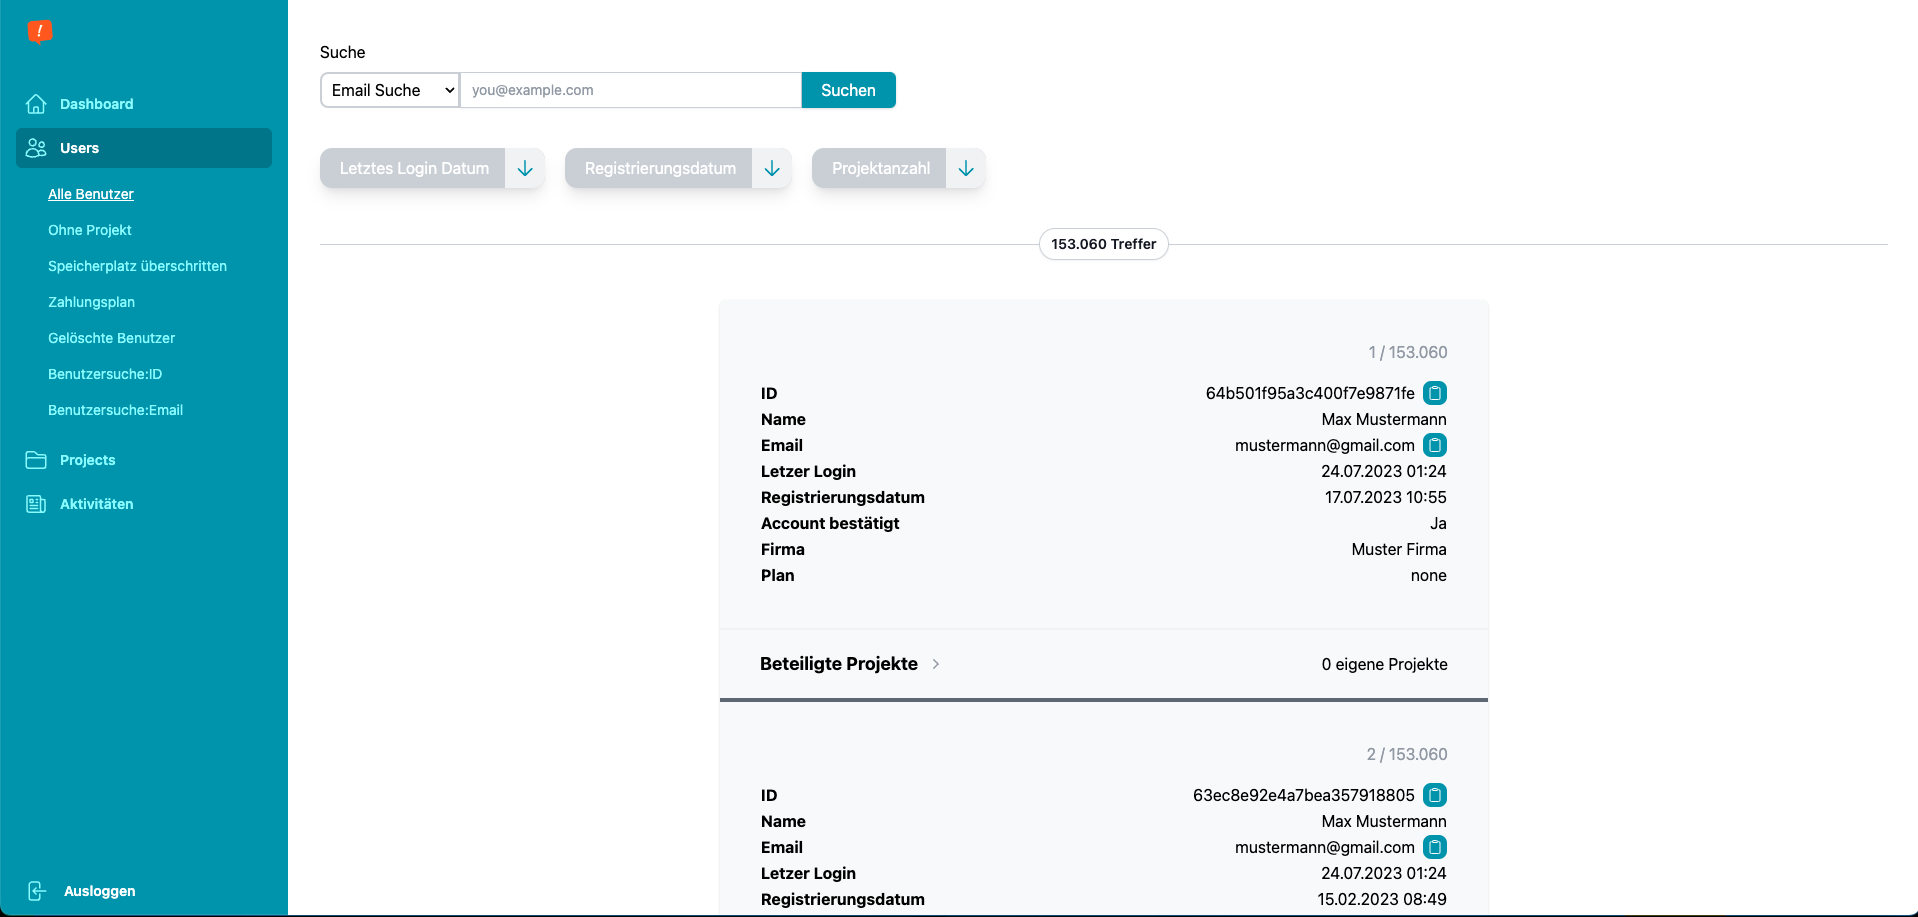
\includegraphics[width=1\textwidth]{pics/planfred-ui-ux-example.png}
    \caption{Kundenmanagement Tool Beispiel}
    \label{fig:mesh1}
\end{figure}

Wir haben hierbei die blauen Farben gezielt verwendet um wichtige Bereiche und Funktionen hervorzuheben. Wie anhand des Screenshotes erkennbar ist, wird die seitliche Navigationbar durch die blaue Farbe hervorgehoben. Der andere Teil der seite, wo der tatsächliche Content zu sehen ist ist im Gegensatz eher hell und simpel gehalten. Dabei wird der Hintergrund weiß eingefärbt und die Daten in grauen Boxen davon getrennt. Das ist zwar sehr minimalistisch, grenzt jedoch trotzdem die verschiedenen Bereiche voneinander ab.

Ebenfalls wurde die blaue Farbe für sogenannte Action Buttons verwendet, also Buttons oder Elemente, die eine Aktion ausführen. Diese stechen damit mehr raus und übermitteln den Benutzer:in, dass diese Elemente eine Funktion haben und nicht nur zur Anzeige dienen.

